\subsection{UCS1 - Importazione dei dati}
\label{sub:ucs1}

%TODO: Add correct image
% Se uno use case esce dalla post allora non mettiamo in scenario secondario ma in estensione
% se invece la post rimane la stessa non è estensione.

\begin{figure}[h]
	\centering
	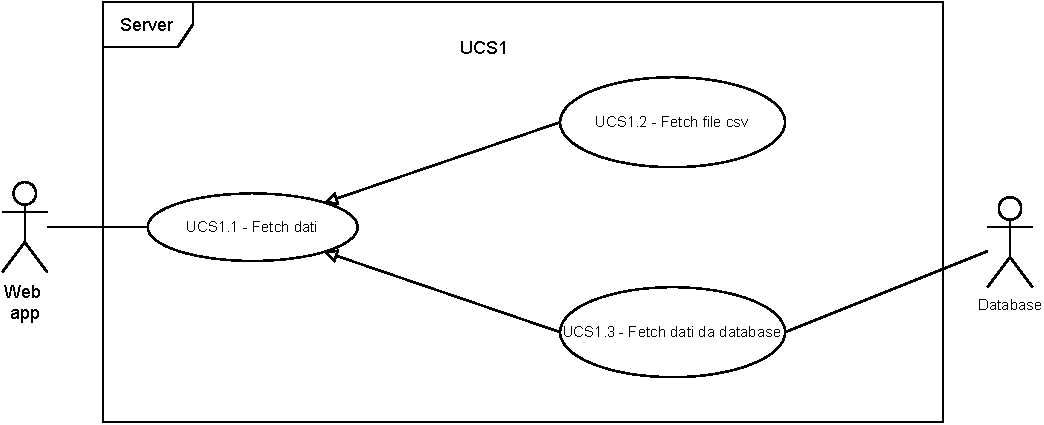
\includegraphics[width=0.7\textwidth]{diagrammi/UCS1.pdf}
	\caption{Diagramma rappresentante UCS1}
	\label{fig:UCS1}
\end{figure}

\begin{itemize}
	\item \textbf{Descrizione}: La Web App comunica la scelta della fonte dei dati al server che si occupa di importare i dati e di dare automaticamente un metadato di tipo e visibilità ai campi del dataset.

	\item \textbf{Attore primario}: Web App;
	\item \textbf{Attore secondario}: Database;

	\item \textbf{Precondizione}:   La fonte dei dati è stata selezionata(\hyperref[ssub:ucw2]{UCW2});

	\item \textbf{Postcondizione}:  Viene caricato il dataset con i metadati generati e vengono comunicati alla web app;

	\item \textbf{Scenario principale}:
	      \begin{enumerate}
		      \item La web app comunica al server la fonte selezionata;
		      \item Il server fa il fetch dei dati e costruisce il dataset;
		      \item Il server genera i metadati di tipo per il dataset.
	      \end{enumerate}

\end{itemize}

\subsubsection{UCS1.1 - Fetch dei dati}
\label{ssub:ucs1.1}

\begin{itemize}

	\item \textbf{Descrizione}: La Web App comunica la scelta della fonte e il server fa il fetch dei dati.

	\item \textbf{Attore primario}: Web App;
	\item \textbf{Attore secondario}: Database;

	\item \textbf{Precondizione}:   La fonte dei dati è stata selezionata (\hyperref[ssub:ucw2]{UCW2});

	\item \textbf{Postcondizione}:  Viene caricato il dataset con i metadati generati e vengono comunicati alla web app;

	\item \textbf{Scenario principale}:
	      \begin{enumerate}
		      \item La web app comunica al server la fonte selezionata;
		      \item Il server fa il fetch dei dati e costruisce il dataset.
	      \end{enumerate}

\end{itemize}


\subsubsection{UCS1.2 - Fetch dei dati da file csv}
\label{ssub:ucs1.2}

\begin{itemize}

	\item \textbf{Descrizione}: La Web App comunica la scelta di usare come fonte un file csv e il server fa il fetch dei dati.

	\item \textbf{Attore primario}: Web App;

	\item \textbf{Precondizione}:   La fonte di dati selezionata è il file csv (\hyperref[ssub:ucw2]{UCW2});

	\item \textbf{Postcondizione}:  Viene caricato il dataset desiderato  e vengono comunicati i dati alla web app;

	\item \textbf{Scenario principale}:
	      \begin{enumerate}
		      \item La web app comunica al server al decisione di usare un file csv;
		      \item Il server fa il fetch dei dati e costruisce il dataset.
	      \end{enumerate}

	\item \textbf{Estensioni}:
	      \begin{itemize}

		      \item Se il file è malformato o vuoto:
		            \begin{enumerate}

			            \item Il caricamento dei dati viene interrotto;
			            \item Viene visualizzato un messaggio di errore(\hyperref[sub:ucw6]{UCW6}).

		            \end{enumerate}

	      \end{itemize}

\end{itemize}

\begin{figure}[h]
	\centering
	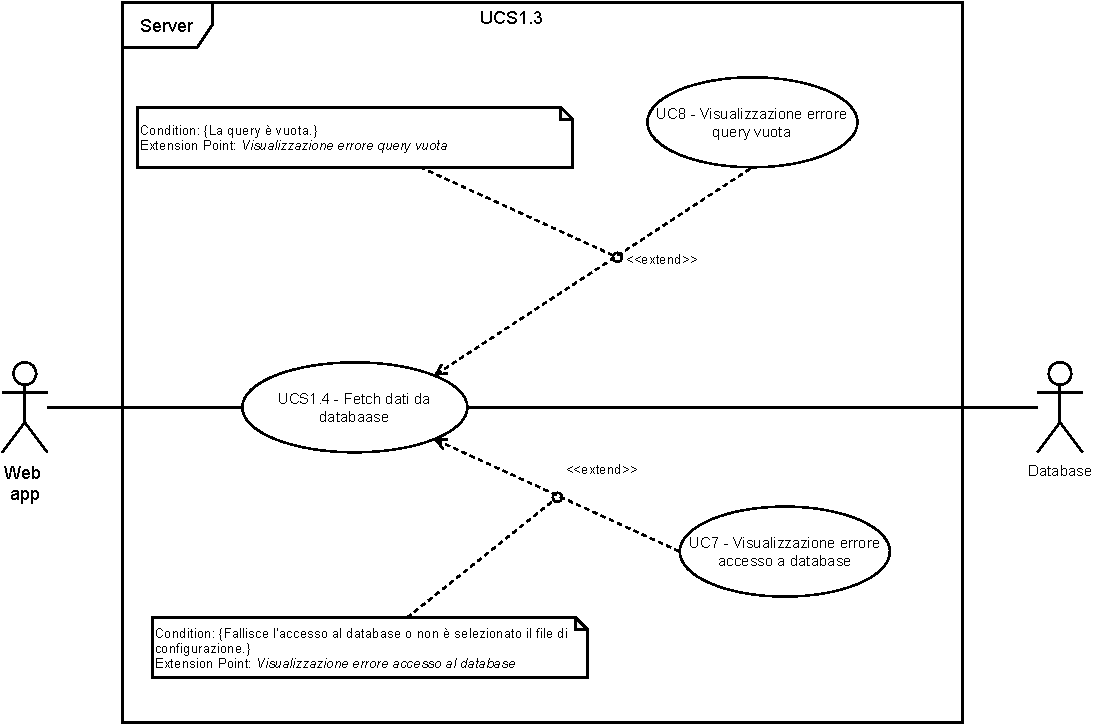
\includegraphics[width=0.7\textwidth]{diagrammi/UCS1_3.pdf}
	\caption{Diagramma rappresentante UCS1}
	\label{fig:UCS1_3}
\end{figure}

\subsubsection{UCS1.3 - Fetch dei dati da database}
\label{ssub:ucs1.3}

\begin{itemize}

	\item \textbf{Descrizione}: La Web App comunica la scelta di usare come fonte un database e la particolare configurazione da utilizzare tra quelle
	      rese disponibili dal server. Viene successivamente eseguito il fetch dei dati.

	\item \textbf{Attore primario}: Web App;
	\item \textbf{Attore secondario}: Database;

	\item \textbf{Precondizione}:   La fonte dei dati è un database ed è stata scelta una query (\hyperref[ssub:ucw2.3]{UCW2.3});

	\item \textbf{Postcondizione}:  Viene caricato il dataset desiderato e vengono comunicati i dati alla web app;

	\item \textbf{Scenario principale}:
	      \begin{enumerate}
		      \item La web app comunica al server la decisione di usare un database e la query scelta;
		      \item Il server fa il fetch dei dati e costruisce il dataset.
	      \end{enumerate}

	\item \textbf{Estensioni}:
	      \begin{itemize}

		      \item Se fallisce l'accesso al database:
		            \begin{enumerate}

			            \item Il caricamento dei dati viene interrotto;
			            \item Viene visualizzato un messaggio di errore (\hyperref[sub:ucw7]{UCW7}).

		            \end{enumerate}

		      \item Se la query è vuota:
		            \begin{enumerate}

			            \item Il caricamento dei dati non viene effettuato;
			            \item Viene visualizzato un messaggio di errore (\hyperref[sub:ucw8]{UCW8}).

		            \end{enumerate}

	      \end{itemize}

\end{itemize}